\documentclass{beamer}
%
% Warsaw is a canned beamer theme, for others see  
%  http://en.wikibooks.org/wiki/LaTeX/Presentations#Themes
%
\usetheme{Warsaw}                                      
\usepackage{tikz}                                         % SM Diagramming stuff
\usepackage{listings}                                   % Source code formatting
\usepackage{hyperref}
\usetikzlibrary{automata,positioning}
\hypersetup{colorlinks=true,linkcolor=red}

\begin{document}
%
% Title Page
%
  \begin{frame}
    \frametitle{State Machines}

    \begin{center}
      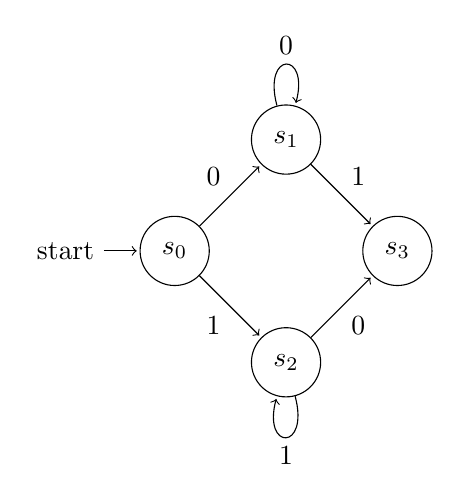
\begin{tikzpicture}[shorten >=1pt,node distance=2cm,on grid,auto] 
        \node[state,initial] (s_0)   {$s_0$}; 
        \node[state] (s_1) [above right=of s_0] {$s_1$}; 
        \node[state] (s_2) [below right=of s_0] {$s_2$}; 
        \node[state](s_3) [below right=of s_1] {$s_3$};
        \path[->] 
        (s_0) edge  node {0} (s_1)
        edge  node [swap] {1} (s_2)
        (s_1) edge  node  {1} (s_3)
        edge [loop above] node {0} ()
        (s_2) edge  node [swap] {0} (s_3) 
        edge [loop below] node {1} ();
      \end{tikzpicture}
      
    \end{center}

November 2013

\end{frame}
%
% Introduction
%
\frame{
  \frametitle{Background}
  \itemize{
    \item Blah! This needs more thought
    \item distinct states 
    \pause
    \item transitions/events
    }
}

  
%
% Why/When/How
%
\frame{
    \frametitle{Why?}
    \framesubtitle{Isn't this academic blather?}
    \itemize{
      \item 
    }
}

\begin{frame}
  \frametitle{When?}  
\end{frame}

\begin{frame}[fragile]
  \frametitle{How?}
\begin{lstlisting}
for (int i = 0; i < 20; i++) {
  // do something
}
\end{lstlisting}

\end{frame}

\frame {
  \frametitle{Small Sampling of State Machine Frameworks}
\href{https://code.google.com/p/stateless4j/}{stateless4j}

%\hyperlink{https://code.google.com/p/stateless4j/}
https://github.com/Beh01der/EasyFlow
https://github.com/hekailiang/squirrel
}

\end{document}
